\documentclass[letterpaper]{article}
\usepackage{aaai}
\usepackage{algorithm}
\usepackage[noend]{algpseudocode}
\usepackage[numbers]{natbib}
\bibliographystyle{plainnat}

\makeatletter
\def\BState{\State\hskip-\ALG@thistlm}
\makeatother

\usepackage{hyperref}
\usepackage{amsmath}
\usepackage{lmodern}
\usepackage{courier}
\usepackage{listings}
\usepackage{graphicx}
\usepackage{tikz}
\usetikzlibrary{bayesnet}
\usetikzlibrary{arrows}
\graphicspath{ {figures/} }

\lstset{basicstyle=\ttfamily\footnotesize,breaklines=true}

\setlength{\pdfpagewidth}{8.5in}
\setlength{\pdfpageheight}{11in}
\pdfinfo{
  /Title (Topic Modeling for Scientific Documents)
  /Author (Jethro Kuan)}
\begin{document}
\nocopyright

\title{Topic Modeling for Scientific Documents}
\author{Jethro Kuan \\
  WING-NUS\\
}
\maketitle
\begin{abstract}
  \begin{quote}
    Topic models are statistical models, used to discover abstract
    topics that occur in a collection of documents. In this paper, we
    focus on the technique of topic modeling, particularly in its
    application to the domain of scientific documents. We discuss
    different approaches to topic modeling, and weigh in on their
    strengths and shortcomings.
  \end{quote}
\end{abstract}

\section{Introduction}
In this information age, the availability of knowledge is
insufficiently met with the tools to navigate it. Archives such as
Arxiv see an exponential growth in the number of documents being
hosted. Developing new tools for browsing, and searching these
documents is a technological challenge that calls for research in
statistical modeling.

Rather than relying on keyword matching, tools like Semantic Scholar
use machine learning to process scientific documents and discover
meaningful structure, empowering researchers to discover papers more
relevant to their work. One such statistical modeling technique is
topic modeling.

Topic modeling attempts to discover abstract topics within documents.
Topic models capture the intuition that if a document is of a
particular topic, then words from the topic should appear more
frequently.

A topic model trained on a corpora of scientific documents could learn
topics such as ``Neural Networks'', ``Biology'' and ``Medicine''.
Topics attribute a high probability to words that relate to the topic.
For example, a ``Neural Networks'' topic would give attribute a high
probability to ``classifiers'', and a low probability to ``bacteria''.
The quotations around the topics are to make explicit that the labels
are human interpretations of what these topics may be. Topic modeling
is an unsupervised problem, and is often trained on unlabeled data.
Automatic labeling of these topics is an active area of research
\cite{mei2007automatic}, \cite{lau2011automatic}.

\begin{figure}[ht]
  \centering
  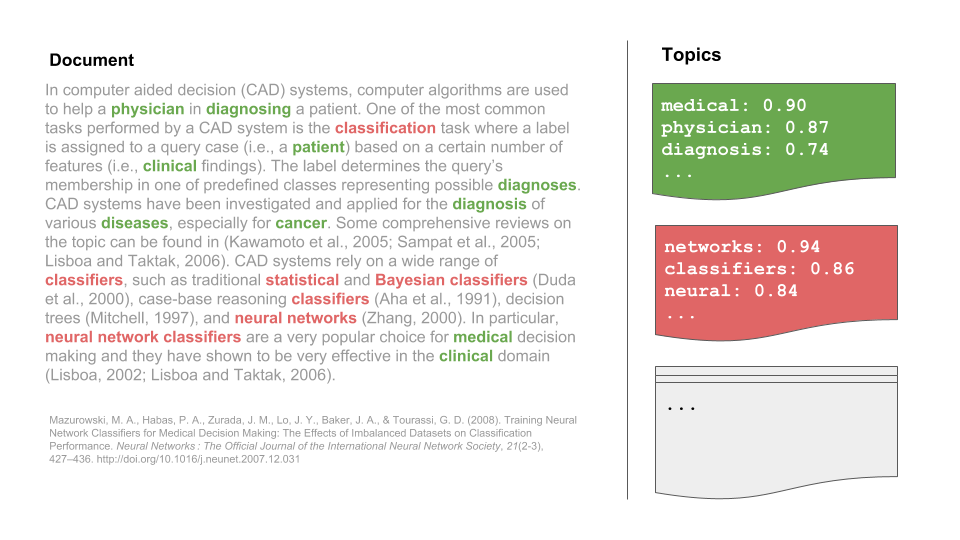
\includegraphics[width=0.5\textwidth]{topic_models.png}
  \caption{\label{fig:topic_model_document} According to the trained
    topic model, topics like ``Medicine'' and ``Neural Networks''
    generate the colored words of the document}
\end{figure}

Topic modeling may discover that document in
~\autoref{fig:topic_model_document} relates to ``Medicine'' and
``Neural Networks'', because these topics give rise to the colored
words in the document.

In addition, we can view these abstract topics as a form of clustering.
Researchers are better able to navigate the large corpora of
scientific knowledge, by exploring documents that have similar topic
proportions.

The earliest known technique for topic modeling is Latent Semantic
Indexing (LSI) \cite{deerwester1990indexing}. The first probabilistic
approach, Probabilistic Latent Semantic Analysis (pLSA), was proposed
in 1999 \cite{hofmann1999probabilistic}. It was only in 2003 when
\citeauthor{blei2003latent} introduced Latent Dirchlet Allocation
(LDA), which remains to this date the predominant technique for topic
modeling.

Most of the state-of-the-art topic models are generative models,
assuming that latent variables govern the generative process of a
document. According to these models, a document is produced from a
distribution of topics, and the topics themselves are distributions
over the vocabulary of the corpora.

In this paper, we briefly discuss the predominant model: Latent
Dirichlet Allocation (LDA) and its variants. In addition, we explore
other models that are not derivatives of LDA, such as the Replicated
Softmax.

\section{LDA}
Latent Dirichlet Allocation is widely considered to be the simplest
topic model. LDA models each document as a mixture of topics, where a
topic $\beta_k$ is a probability distribution over a fixed vocabulary
of terms. Training LDA requires fixing the number of topics, $K$.
We can draw the graphical model for LDA as in
~\autoref{fig:lda_plate}.

At risk of being pedantic, we explain the graphical model in detail.
$\eta$ is the topic hyperparameter, which produces a topic
distribution $\beta_k$ of the Dirichlet family. There are a total of
$K$ topics. Similarly, $\alpha$ is a hyperparameter that produces the
per-document topic proportions $\theta_d$. These Dirichlet
distributions are of dimension $K-1$, because there are a total of $K$
topics. There are $D$ such topic proportions, where $D$ is the total
number of documents. $Z_{d,n}$ is the per-word topic assignment, drawn
from the particular $\theta_d$. Finally, $W_{d,n}$ is the $n$th word
in the $d$th document, an observed variable. It is simple to see that
$P(W_{d,n} | Z_{d,n}, \beta_{k}) = \beta_{z_{d,n}, w_{d,n}}$.

A high $\alpha$ value encodes the belief that documents contain a
mixture of many topics, rather than being largely represented by a few
topics. Similarly, a high $\eta$ value encodes the belief that topics
has high probability for a large number of words in the vocabulary.

\begin{figure}[ht]
  \centering
  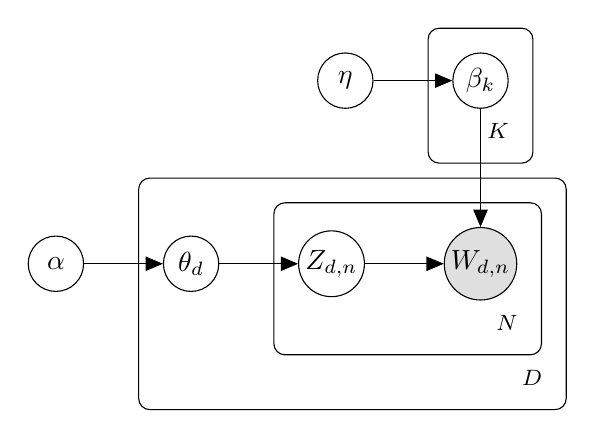
\begin{tikzpicture}
    \node[latent] (a) {$\alpha$};
    \node[latent, right=of a] (t) {$\theta_d$};
    \node[latent, right=of t] (z) {$Z_{d,n}$};
    \node[obs, right=of z] (w) {$W_{d,n}$};
    \node[latent, above=1.5cm of w] (b) {$\beta_k$};
    \node[latent, left=of b] (e) {$\eta$};

    % Edges
    \edge {a} {t};
    \edge {t} {z};
    \edge {z} {w};
    \edge {e} {b};
    \edge {b} {w};

    % Plates
    \plate [inner sep=0.3cm] {pN} {(z)(w)} {$N$};
    \plate [inner sep=0.3cm] {pM} {(t)(z)(w)(pN)} {$D$};
    \plate [inner sep=0.3cm] {pK} {(b)} {$K$};
  \end{tikzpicture}
  \caption{\label{fig:lda_plate} Plate notation for LDA.}
\end{figure}

We can fully specify the model by looking at the joint distribution
$\mathcal{J}$ of all the latent and observed variables.

\begin{multline}
 \mathcal{J} = \left( \sum_{k=1}^{K} P(\beta_k | \eta) \right) \left(
    \sum_{d=1}^{D} P(\theta_d | \alpha) \right) \\
  \left( \sum_{n=1}^{N} \theta_{d, Z_{d,n}} \beta_{Z_{d,n}, W_{d,n}} \right)  
\end{multline}

The generative process of a document is as follows:

\begin{algorithm}
  \caption{Generative Process of LDA}\label{alg:LDA}
  \begin{algorithmic}[1]
    \For {each document $d$ in $D$}
    \State {Draw topic distribution $\theta_d \sim Dir(\alpha)$}
    \For {each word $n_d$ in $N_d$}
    \State {Sample topic $z_{d,n} \sim Multinomial(\theta)$}
    \State {Sample word $w_{d,n} \sim Multinomial(\beta_{z_{d,n}})$}
    \EndFor
    \EndFor
  \end{algorithmic}
\end{algorithm}

If we fix the topic distributions $\beta_{1:K}$, we can compute the
per-document posterior $\theta$ given the document.

\begin{multline}
  P(\theta | w_{1:n}, \alpha, \beta_{1:K}) = \\ \frac{P(\theta |
    \alpha)\prod_{n=1}^{N} P(z_n | \theta) P(w_n | z_n,
    \beta_{1:K})}{\int_\theta P(\theta | \alpha) \prod_{n=1}^N
    \sum_{z=1}^K P(z_n | \theta) P(w_n | z_n, \beta_{1:K})}
\end{multline}


The denominator is intractable to compute, due to the coupling
between $\theta$ and $\beta$ under the multinomial assumption.
\cite{blei2003latent}. Hence, we rely on techniques for approximate
inference of the posterior. We discuss these techniques in
~\autoref{sec:inference}.

Why does LDA work? The Dirichlet distribution encourages sparsity,
encoding the belief that the document-topic distribution has few
topics per document, and the topic-word distribution has few words per
topic. These two beliefs work against each other, and LDA discovers
this sparsity balance, which gives rise to the structure of the
textual data.

\subsection{Statistical Assumptions}
\label{subsec:statistical-assumptions}
As Mackay quips, we cannot make inference without statistical
assumptions. LDA makes several assumptions, some rendering it less
suited for application to the domain of scientific documents.

LDA models documents as ``bag-of-words'': words within the document
are interchangeable. \cite{blei2003latent} I think this is a
reasonable assumption to make, given the task is to discover themes
within the document.

LDA also assumes that the order of documents do not matter.
Exchangeability of both words and documents allows LDA to model the
joint distribution as a mixture model. I believe this assumption to be
invalid in the domain of scientific documents. The meaning of
keyphrases used in scientific literature change over time. For
example, the landscape of research neural networks is vastly different
now, as compared to the 1990s, and LDA will fail to capture these
differences.

The use of the Dirichlet distribution also encodes statistical
assumptions about the correlation between topics. Under the Dirichlet,
components of $\theta_d$ are nearly independent. This leads to the
modeling assumption that the presence of one topic is not correlated
with the presence of another \cite{blei2007correlated}. As explained
by \citeauthor{blei2007correlated}, this assumption is strong and
unrealistic in the domain of scientific documents. An article about
genetics is also highly likely to be about health and disease, and
unlikely to be about astronomy \cite{blei2007correlated}.

Variants of LDA relax these statistical assumptions, or make other
assumptions in place. We discuss Dynamic Topic Modeling (DTM) in
~\autoref{sec:dtm} and Correlated Topic Modeling(CTM), and briefly
mention the rest in the appendix.

\section{Correlated Topic Modeling}
\label{sec:ctm}
The Correlated Topic Model (CTM) addresses the model assumption that
topic proportions are not correlated. In scientific documents, this
assumption is unlikely to hold true.

Instead of drawing from a Dirichlet distribution, the CTM uses a
logistic normal distribution. CTM draws a real valued random vector
from a multivariate Gaussian, and maps it to the simplex to obtain a
multinomial parameter \cite{blei2007correlated}. The $K \times K$
covariance matrix $\Sigma$ models dependencies between the topics.
This tweak is evident in the generative process shown in Algorithm
~\autoref{alg:CTM}, contrasting it with Algorithm ~\autoref{alg:LDA}.

\begin{algorithm}
  \caption{Generative Process of CTM}\label{alg:CTM}
  \begin{algorithmic}[1]
    \For {each document $d$ in $D$}
    \State {Draw topic distribution $\beta_d \sim \mathcal{N}(\mu, \Sigma)$}
    \For {each word $n_d$ in $N_d$}
    \State {Sample topic $z_{d,n} \sim Multinomial(\pi(\beta_d))$}
    \State {Sample word $w_{d,n} \sim Multinomial(\beta_{z_{d,n}})$}
    \EndFor
    \EndFor
  \end{algorithmic}
\end{algorithm}

$\pi$ maps the multinomial parameters to the mean parameters,
$\pi\left( x \right) = \frac{e^x}{\sum_{i} e^{x_i}}$

We can also visualize CTM with a graphical model.

\begin{figure}[ht]
  \centering
  \begin{tikzpicture}
    \node[latent] (S) {$\Sigma$};
    \node[latent, left= of t, yshift=-1cm] (m) {$\mu$};
    \node[latent, right= of S, yshift=-0.5cm] (t) {$\theta_d$};
    \node[latent, right=of t] (z) {$Z_{d,n}$};
    \node[obs, right=of z] (w) {$W_{d,n}$};
    \node[latent, above=1.5cm of w] (b) {$\beta_k$};
    \node[latent, left=of b] (e) {$\eta$};

    % Edges
    \edge {S} {t};
    \edge {m} {t};
    \edge {t} {z};
    \edge {z} {w};
    \edge {e} {b};
    \edge {b} {w};

    % Plates
    \plate [inner sep=0.3cm] {pN} {(z)(w)} {$N$};
    \plate [inner sep=0.3cm] {pM} {(t)(z)(w)(pN)} {$D$};
    \plate [inner sep=0.3cm] {pK} {(b)} {$K$};
  \end{tikzpicture}
  \caption{\label{fig:ctm_plate} Plate notation for CTM.}
\end{figure}


The Multinomial and Guassian distributions are not conjugate
distributions. This causes inference via Gibbs sampling is difficult.
Hence, variational inference is used instead.


\section{Dynamic Topic Modeling}
\label{sec:dtm}
Dynamic Topic Modeling (DTM) was proposed to remove the assumption
that documents are \textit{exchangeable}. \cite{blei2006dynamic}

The order of documents are important for scientific documents, since
both the content, and the meaning of words evolve over time.

In DTM, data is divided by discrete time slices. The topics associated
with time slice $t$ evolve from the time slice $t-1$. Because the
Dirichlet distribution is not amenable to sequential modeling, we use
the Gaussian distribution to model the sequence of random variables.

The generative process for time slice $t$ is as follows:

\begin{algorithm}
  \caption{Generative Process of DTM}\label{alg:DTM}
  \begin{algorithmic}[1]
    \State {Draw topic distribution $\beta_t | \beta_{t-1} \sim N(\beta_{t-1},
  \sigma^2I)$}
    \State {Draw $\alpha_t | \alpha_{t-1} \sim N\left( \alpha_{t-1}, \delta^2I
    \right)$}
    \For {each document $w$}
    \State {Draw $\eta_{w,t} \sim N\left( \alpha_t, a^2I \right)$}
    \For {each word at position $n$}
    \State {Sample topic $z_{t,n} \sim Multinomial(\pi(\eta_{w,t}))$}
    \State {Sample word $w_{t,d,n} \sim Multinomial(\beta_{t,z,n})$}
    \EndFor
    \EndFor
  \end{algorithmic}
\end{algorithm}

\begin{figure}[ht]
  \centering
  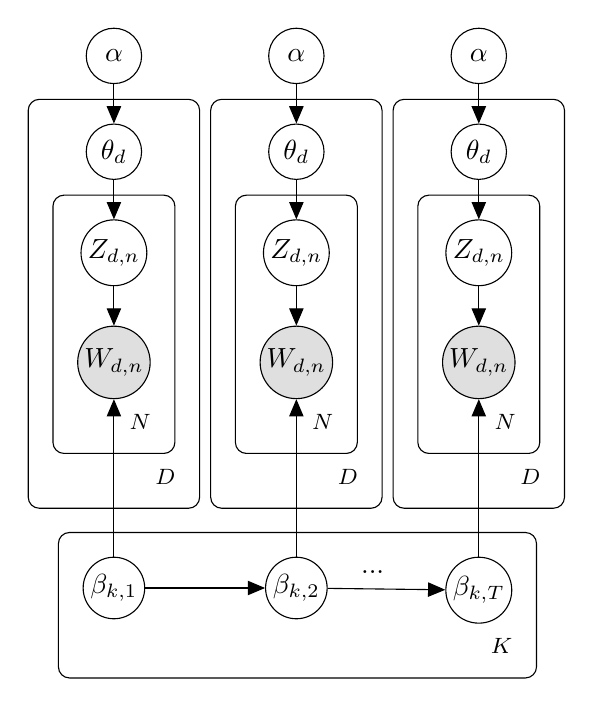
\begin{tikzpicture}
    \node[latent] (a1) {$\alpha$};
    \node[latent, below=0.5cm of a1] (t1) {$\theta_d$};
    \node[latent, below=0.5cm of t1] (z1) {$Z_{d,n}$};
    \node[obs, below=0.5cm of z1] (w1) {$W_{d,n}$};
    \node[latent, below=2cm of w1] (b1) {$\beta_{k,1}$};

    \node[latent, right=1.6cm of a1] (a2) {$\alpha$};
    \node[latent, below=0.5cm of a2] (t2) {$\theta_d$};
    \node[latent, below=0.5cm of t2] (z2) {$Z_{d,n}$};
    \node[obs, below=0.5cm of z2] (w2) {$W_{d,n}$};
    \node[latent, below=2cm of w2] (b2) {$\beta_{k,2}$};

    \node[latent, right=1.6cm of a2] (at) {$\alpha$};
    \node[latent, below=0.5cm of at] (tt) {$\theta_d$};
    \node[latent, below=0.5cm of tt] (zt) {$Z_{d,n}$};
    \node[obs, below=0.5cm of zt] (wt) {$W_{d,n}$};
    \node[latent, below=2cm of wt] (bt) {$\beta_{k,T}$};

    % Edges
    \edge {a1} {t1};
    \edge {t1} {z1};
    \edge {z1} {w1};
    \edge {b1} {w1};

    \edge {a2} {t2};
    \edge {t2} {z2};
    \edge {z2} {w2};
    \edge {b2} {w2};

    \edge {at} {tt};
    \edge {tt} {zt};
    \edge {zt} {wt};
    \edge {bt} {wt};

    \edge {b1} {b2};
    \edge {b2} {bt};
    \node[text=, right=0.3cm of b2, yshift=0.2cm] {...};

    % Plates
    \plate [inner sep=0.3cm] {pN1} {(z1)(w1)} {$N$};
    \plate [inner sep=0.3cm] {pM1} {(t1)(z1)(w1)(pN1)} {$D$};

    \plate [inner sep=0.3cm] {pN2} {(z2)(w2)} {$N$};
    \plate [inner sep=0.3cm] {pM2} {(t2)(z2)(w2)(pN2)} {$D$};

    \plate [inner sep=0.3cm] {pNt} {(zt)(wt)} {$N$};
    \plate [inner sep=0.3cm] {pMt} {(tt)(zt)(wt)(pNt)} {$D$};
    
    \plate [inner sep=0.3cm] {pK} {(b1)(b2)(bt)} {$K$};
  \end{tikzpicture}
  \caption{\label{fig:lda_plate} Plate notation for DTM.}
\end{figure}

Similar to CTM, the use of the logistic normal distribution causes
variational inference to be the preferred approximate inference
technique.

Further extensions of this approach include the continuous Dynamic
Topic Models (cDTM), which removes the discretization of the time
slices. \cite{wang-2012-contin-time} This model has been used to
predict the timestamp of documents.

\section{Bayesian Non-parametric Models}
One important component we have yet to discuss is the choice of $K$,
the number of topics used to model the corpora. Notice that the value
of $K$ affects model complexity. LDA, CTM and DTM are Bayesian
parametric models: documents are modeled as mixtures of $K$
distributions. The choice of $K$ is therefore also an important
parameter that requires tuning. This is a pitfall of parametric
models. A misfit between the complexity of the model and the amount
and quality of data available can lead to severe underfitting or
overfitting \cite{teh2011dirichlet}.

Bayesian non-parametric models provide an elegant solution to this
issue. The non-parametric approach allows the model to grow in
complexity as more data is observed. These non-parametric models have
also been extended to hierarchies of topics, moving from more general
to more concrete \cite{blei2010nested}.

Bayesian non-parametric models has seen some success in
recommendation systems \cite{gopalan2014bayesian}, a popular modeling
technique in production systems because of its ability to adapt with
growing data size.

\section{Inference Methods}
\label{sec:inference}
Approximating intractable probability densities is a well-studied
problem in modern statistics. This problem arises often in Bayesian
statistics, where computing posterior probablity densities in requires
inference over latent variables. Many learning algorithms have been
developed, including collapsed Gibbs Sampling, Variational Inference,
Collapsed Variational Inference, and MAP estimation. Each of these
approximation techniques have their own strength and shortcomings.

The two inference methods are briefly discussed below, and a
comparison between them relegated to the appendix in
~\autoref{sub:choosing-inference}.

\subsection{MCMC Sampling}
\label{subsec:mcmc-sampling}
Historically, Markov Chain Monte Carlo (MCMC) sampling has been the
dominant technique for approximating posterior densities. In MCMC, we
construct an ergodic Markov chain on the latent variable $z$,
whose stationary distribution is the posterior $P( z | x)$.
Samples are drawn from the stationary distribution, and used to
approximate the posterior empirically.

In Gibbs sampling, the space of the Markov Chain is the space of the
configurations of the hidden variables. In Gibbs sampling, the next
state is reached by sequentially sampling all variables from the
distribution, conditioned on all the current sampled values. After a
``burn-in'' period, the samples would be drawn from the posterior
distribution.

\begin{algorithm}
\caption{Gibbs Sampling}\label{alg:gibbs}
\begin{algorithmic}[1]
  \State $x^{0}$ $\gets$ $q(x)$
  \For {$i = 1, 2, 3, \hdots$}
  \For {$d = 1, 2, 3, \hdots, D$}
  \State {$x_d^{i} \sim P(X_1 = x_1 | {X_k} = x_k^{i-1} \text{ for } k
    = \{1..n \setminus d\})$}  
  \EndFor
  \EndFor
\end{algorithmic}
\end{algorithm}

A full treatment of Gibbs Sampling applied to LDA can be found in
\cite{griffiths2002gibbs}.

\subsection{Variational Inference}
\label{subsec:vi}
In variational inference, the posterior distribution over a set of
unobserved variables $p(Z|H)$ is approximated by a distribution
$q(Z)$, selected to be in a family that can approximately model the
true posterior. Inference is performed by minimizing the distance
between $p(Z|H)$ and $q(Z)$. One common metric used is the
KL-divergence. Here, we discuss variational inference for LDA.

Mean field variational inference (MFVI) breaks the coupling between
$\theta$ and $z$ by introducing free variational parameters $\gamma$
over $\theta$ and $\phi$ over $z$ and dropping the edges between them.
This results in an approximate posterior $q(\theta, z | \gamma, \phi)
= q_\gamma(\theta)\prod_nq_\phi(z_n)$. This is illustrated in the
graphical model in \autoref{fig:lda_vi}.

\begin{figure}[ht]
  \centering
  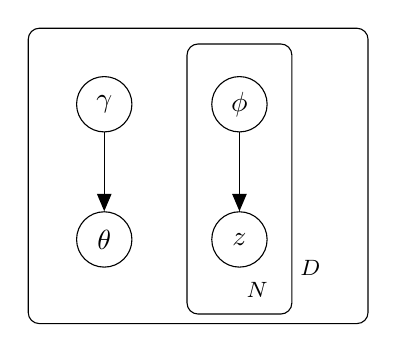
\begin{tikzpicture}
    \node[latent] (y) {$\gamma$};
    \node[latent, below=of y] (t) {$\theta$};
    \node[latent, right=of y] (p) {$\phi$};
    \node[latent, below=of p] (z) {$z$};

    % Edges
    \edge {y} {t};
    \edge {p} {z};
    
    % Plates
    \plate [inner sep=0.3cm, yshift=0.1cm] {pN} {(p)(z)} {$N$};
    {\tikzset{plate caption/.append style={right=0.4cm of #1.south
          east}} \plate [inner sep=0.6cm] {pD} {(y)(t)(p)(z)} {$D$}};
  \end{tikzpicture}
  \caption{\label{fig:lda_vi} Graphical model for the approximate
    posterior for variational inference.}
\end{figure}

To best approximate the true posterior, we frame it as an optimization
problem, minimizing $L$ where:

\begin{equation}
L(\gamma, \phi | \alpha, \beta) = D_{KL}\left[ q(\theta, z | \gamma,
  \phi) || p(\theta, z | \alpha, \beta) \right] - \log p(w | \alpha, \beta)
\end{equation}

This optimization has closed form coordinate descent equations for
LDA, because the Dirichlet is conjugate to the Multinomial
distribution. This computational convenience comes at the expense of
robustness, making it difficult to apply to other more complicated
topic models \cite{blei2003latent}. 

\subsection{Choosing an Inference Method}
\label{sub:choosing-inference}
How do we know which technique to use to approximate the posterior
density? MCMC methods are computationally more intensive, but provide
samples that are approximately exact from the target posterior
density. In contrast, VI methods view the problem as an optimization
problem, which allows it to utilize efficient learning algorithms such
as stochastic optimization. This is much quicker to compute, and is
suited for larger datasets.

However, MCMC methods, cover a large family of sampling methods.
Gibbs sampling requires that the prior and posterior are conjugate
distributions. When this is not possible, such as in DTM, VI methods
can perform better than other methods in the MCMC family.

A closer look at the different inference approximation algorithms,
however, shows that the performance differences can be explained away
by setting certain smoothing hyperparameters
\cite{asuncion-2012-smoot-infer}.

\section{Experimental Results}

\section{Critique of Models and Results}
Both DTM and CTM show that LDA is promising as a base model that can
be adapted to the problem domain. This can be attributed to the
simplicity of LDA. Bayesian non-parametric models

The evaluation of topic models is also an area of research that is
relatively unexplored. The unsupervised nature of topic modeling makes
model selection difficult: there are no gold labels for topics, and
document topic proportions. The most common evaluation metric is the
probability of held-out documents given a trained model
\cite{wallach2009evaluation}, and we refer you to
\citeauthor{wallach2009evaluation} for a full treatment .

\section{Conclusion}
In this paper, we have discussed the importance of topic modeling, and
the opportunities it presents in the domain of scientific documents.
LDA is widely regarded as the simplest topic model, which operates on
the intuition that a document has few topics, and a topic has few
words. LDA is popular as a building block for other topic models. We
discussed the statistical assumptions that LDA makes, and how
appropriate they are in the context of scientific documents. CTM and
DTM were introduced in detail, in the context of relaxing statistical
assumptions made by LDA. We also discussed the difficulties faced in
evaluating the models, that arise from the unsupervised nature of the
problem.

To compare the model outputs, we trained the three models on the ACM
dataset, and presented the topic distributions of each model.

\section{Future Work}
The topic models we have surveyed are directed graphical models.
Despite the recent discoveries in deep learning, LDA, which is over a
decade old, has not yet been replaced as the mainstay for topic
modeling. Deep generative models in particular hold much promise, and
is seeing some recent development \cite{hinton2009replicated,
  larochelle2012neural}. In future we hope to explore this area.

\bibliography{survey}
\end{document}
